\documentclass[]{article}
\usepackage[a4paper, total={6in, 10in}]{geometry}
\usepackage{hyperref}
\usepackage{amsmath}
\usepackage{graphicx}
\usepackage[outdir=./]{epstopdf}
\usepackage{booktabs}
\usepackage{float}
\usepackage{subcaption}

\setlength{\parindent}{0em}
\setlength{\parskip}{1em}

\DeclareMathOperator{\cov}{cov}

%opening
\title{SSY 230, System Identification\\
	Project 1: Estimating functions from noisy data}
\author{Yuxuan Xia\\ \href{mailto:yuxuan.xia@chalmers.se}{yuxuan.xia@chalmers.se}\\Emil Staf\\\href{mailto:emil.staf@chalmers.se}{emil.staf@chalmers.se}}

\begin{document}

\maketitle


\section{Flexible Robot Arm}
The system we have chosen to identify is a mechanical system, where a flexible robot arm have been installed on an electrcal motor. It is a SISO system where the input $u(t)$ is measured reaction torque and the output $y(t)$ is the acceleration of the flexible robot arm. The experimental set-up was performed using a periodic sinusodial sweep.

\subsection{Data}
As mentioned previously the input data is a periodic sinusodial sweep (see top plot of Figure \ref{fig:input}). Due to the fact that the data was obtained using a periodic sinusodial sweep we split the data in half and use the first part as training data and the second part as validation data.

\begin{figure}[ht]
\centering
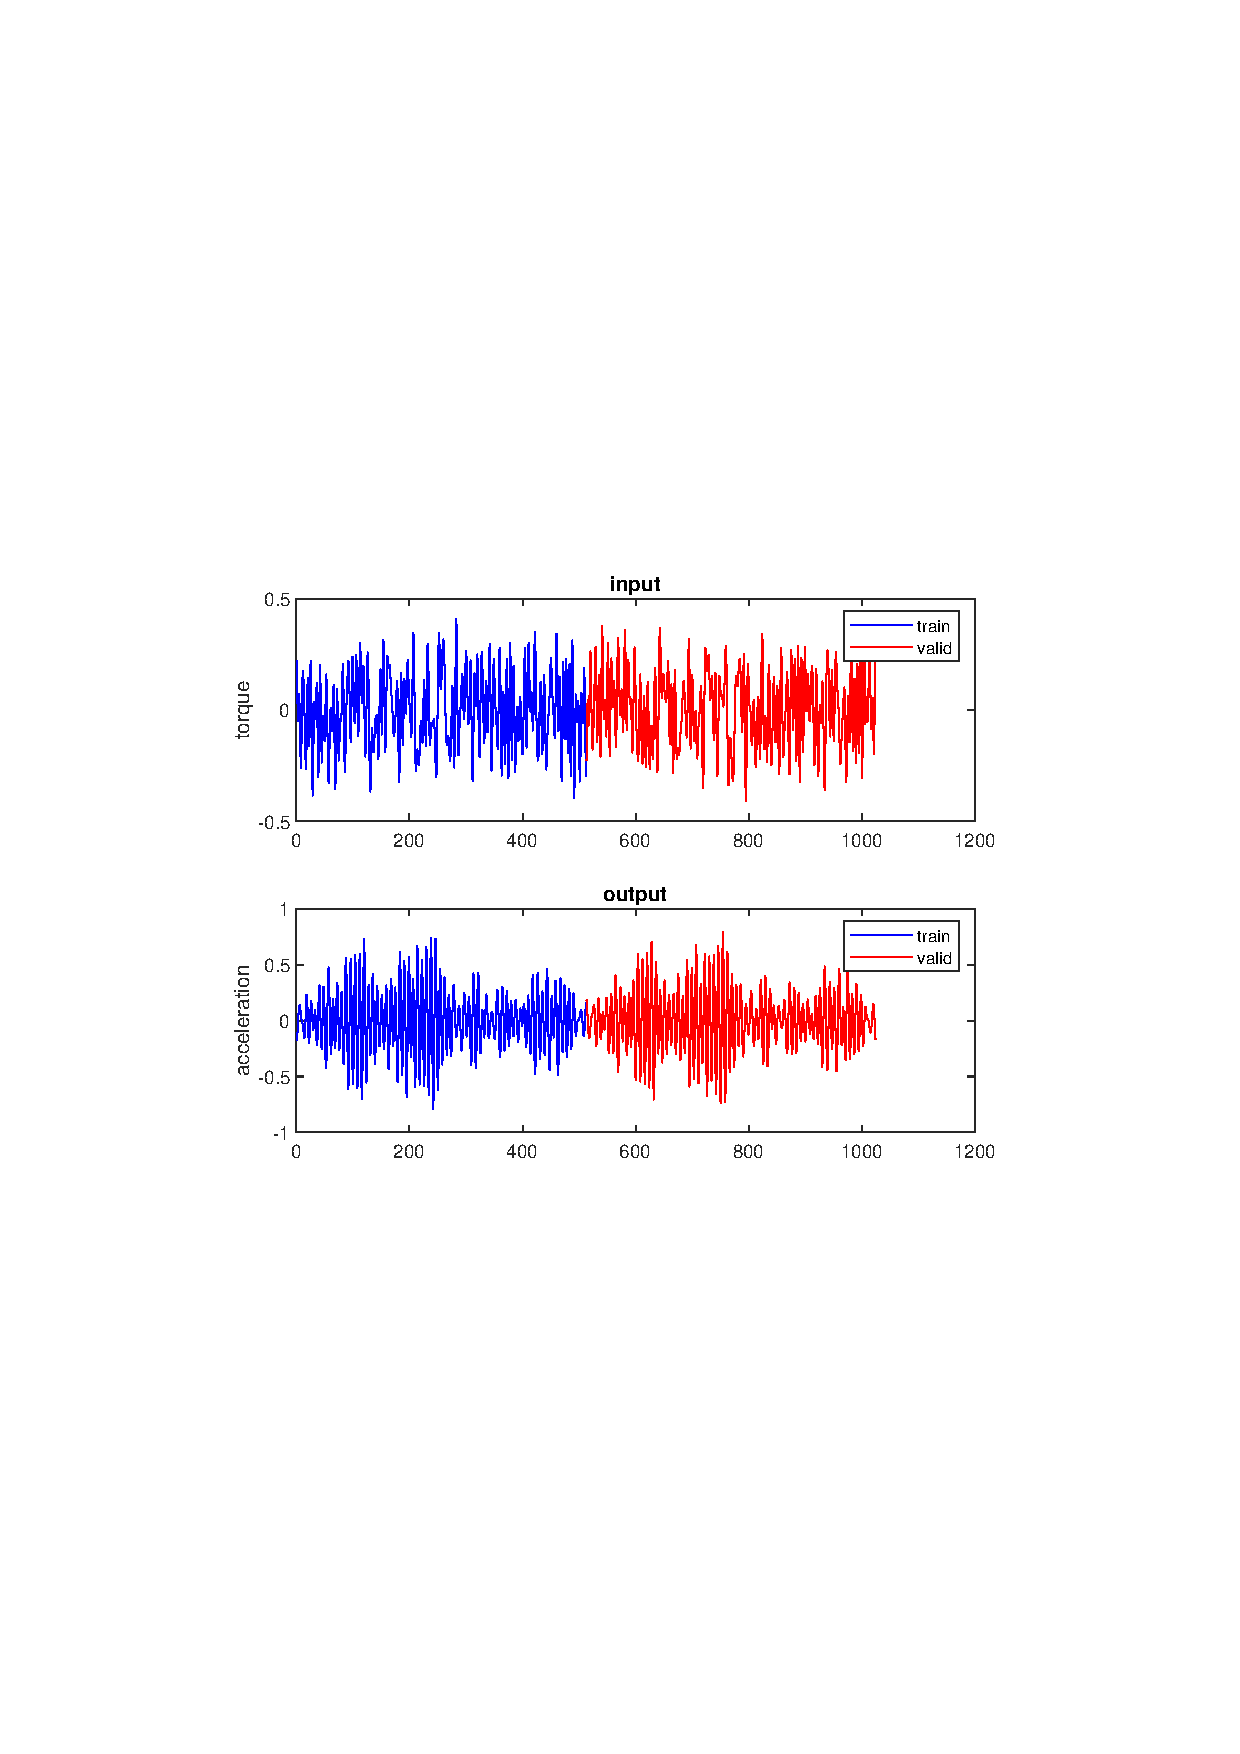
\includegraphics[trim= 10cm 8cm 10cm 8cm, scale=0.6]{figures/input.pdf}
\caption{System data, input $u(t)$ (top) and output $y(t)$ (bottom).}
\label{fig:input}

\end{figure}
To make sure that the frequency content in both the training and validation data are similar we use the \emph{etfe} in MATLAB to find the Empirical Transfer Function Estimate of training- and validation data. The resulting bode-plot is shown in Figure \ref{fig:bode-train_valid}.

\begin{figure}[ht]
\centering
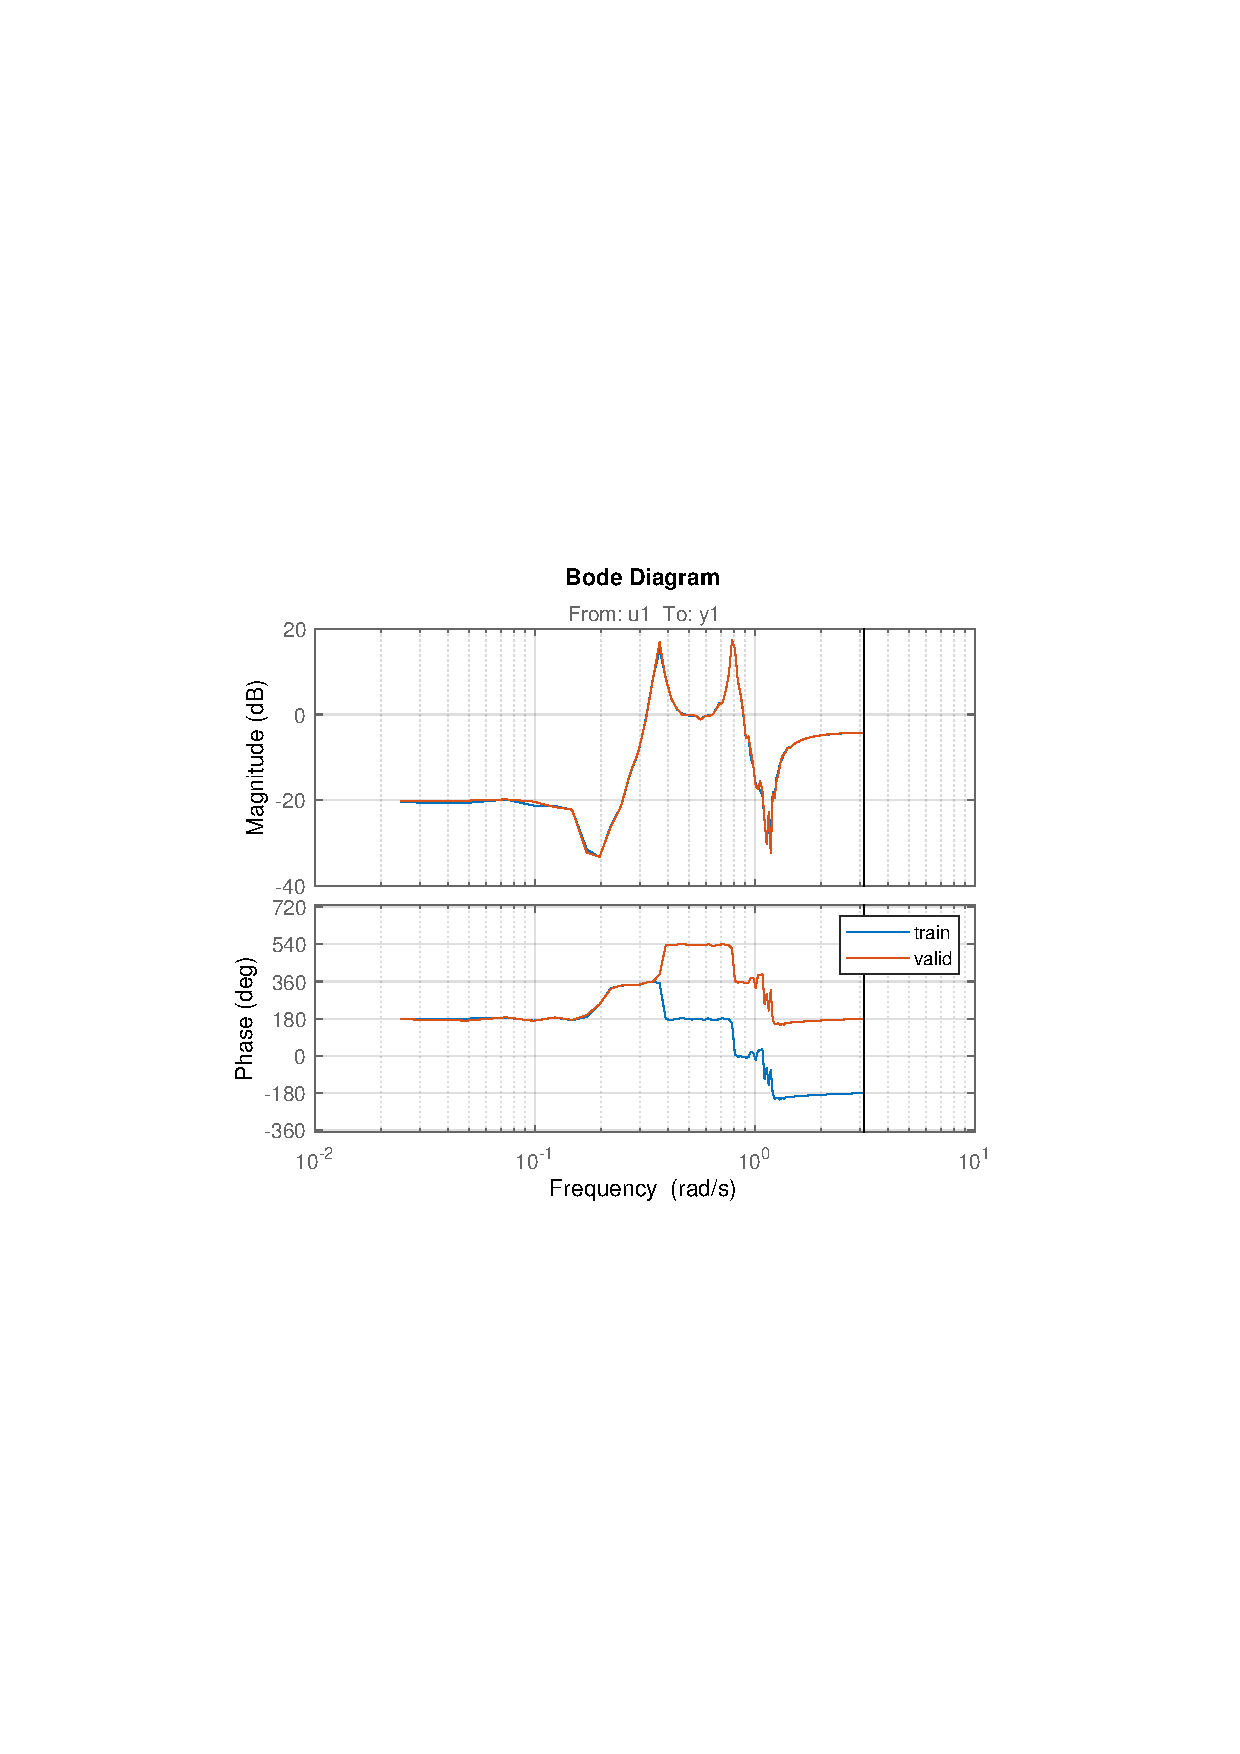
\includegraphics[trim= 10cm 8cm 10cm 8cm, scale=0.6]{figures/bode-train_valid.pdf}
\caption{Bode-plot of training and validation data.}
\label{fig:bode-train_valid}
\end{figure}
From analysing Figure \ref{fig:bode-train_valid} it is clear that the amplitude of the frequency content in both training- and validation data is very similar, while there is a phase shift for frequencies $>0.35$ rad/s.

\subsection{Pre-Processing}

\ifx
\begin{align}
	\label{eq:}
	A(q^{-1})y(t) &= B(q^{-1})u(t) + e(t) \\
	\theta &= (a_1, \ldots a_{na}, b_1, \ldots, b_{nb})^\mathsf{T}
\end{align}


\begin{equation}
	\label{eq:}
	y(t) = \phi(t) \theta + e(t)
\end{equation}


% Figure
\begin{figure}[ht]
\centering
\begin{subfigure}{.49\textwidth}
	\centering
	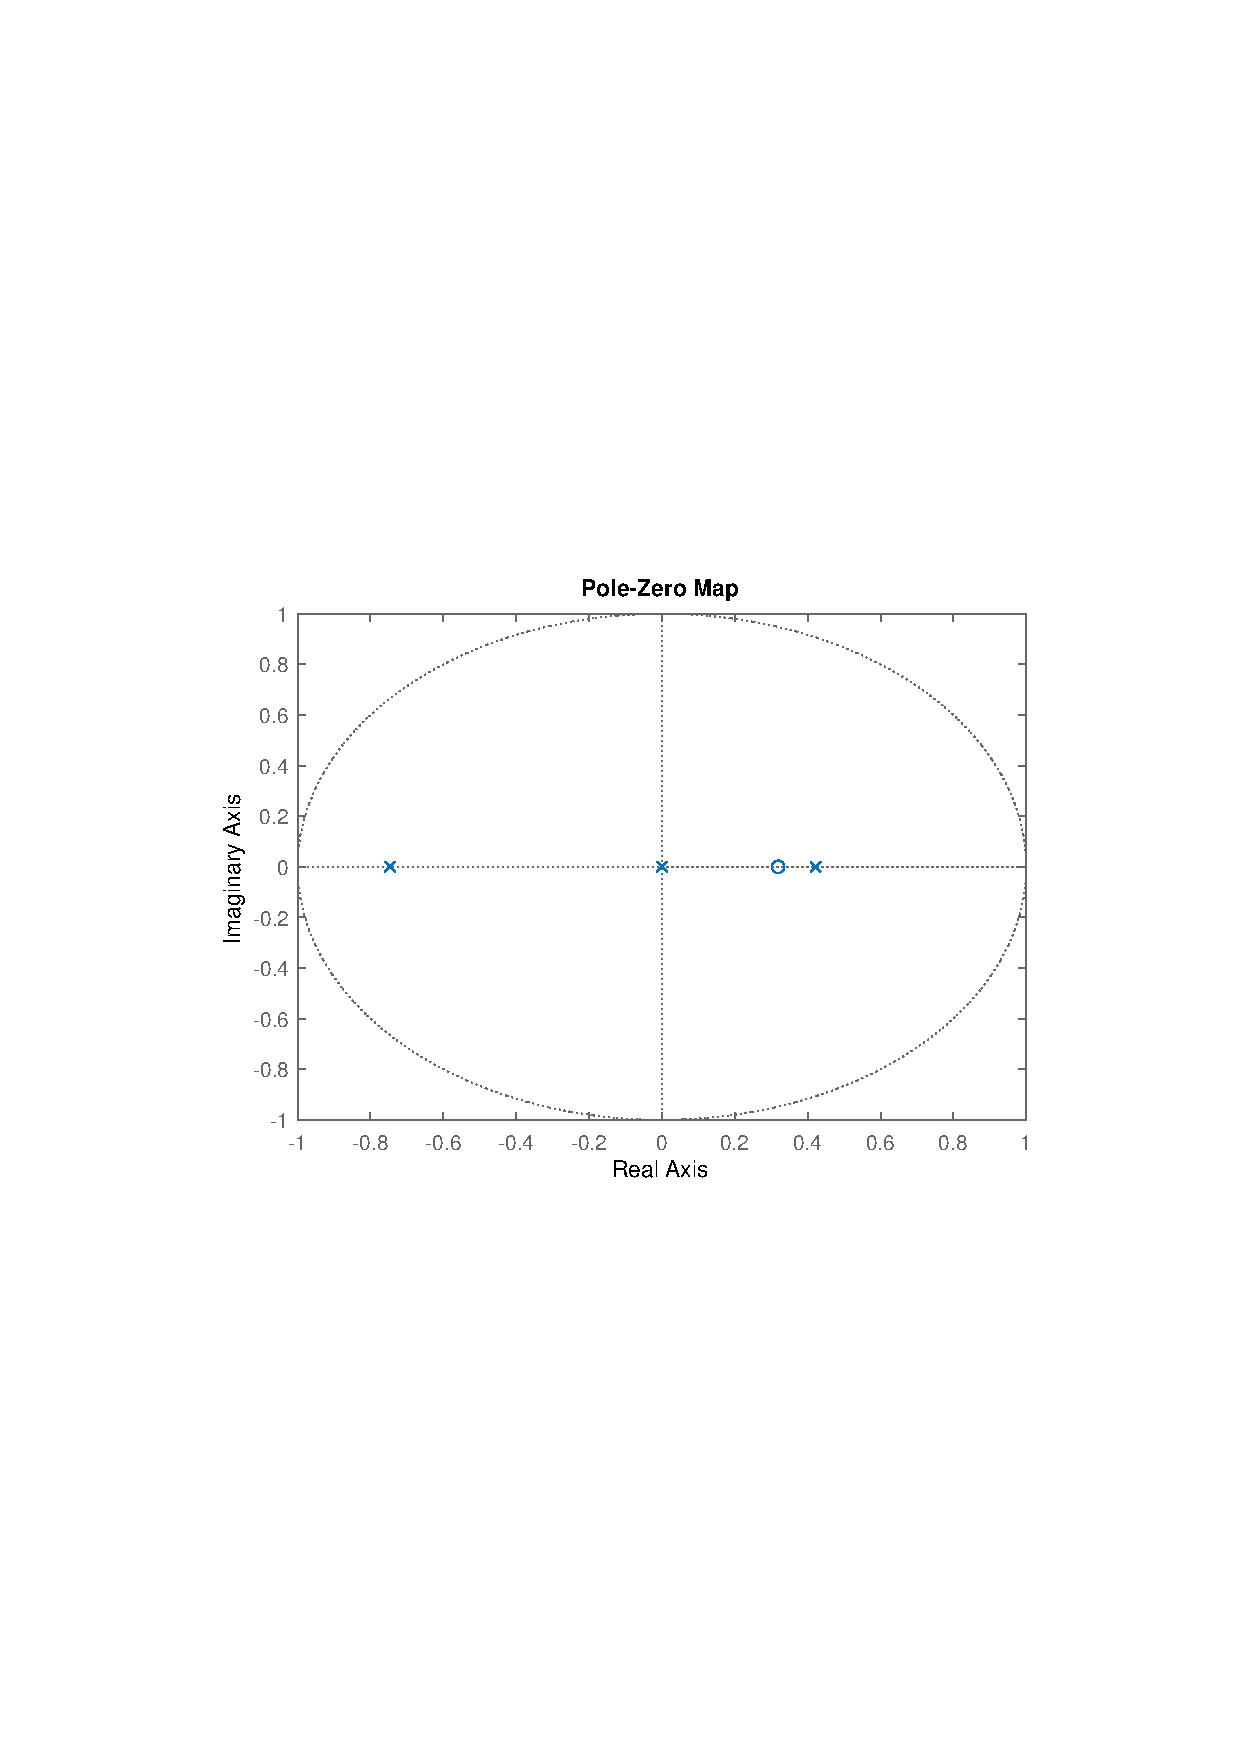
\includegraphics[trim= 10cm 8cm 10cm 8cm, scale=0.4]{figures/1b-pzmap.pdf}
	\caption{pzmap using ltiview}
	\label{fig:1b-pzmap}
\end{subfigure}
\begin{subfigure}{.49\textwidth}
	\centering
	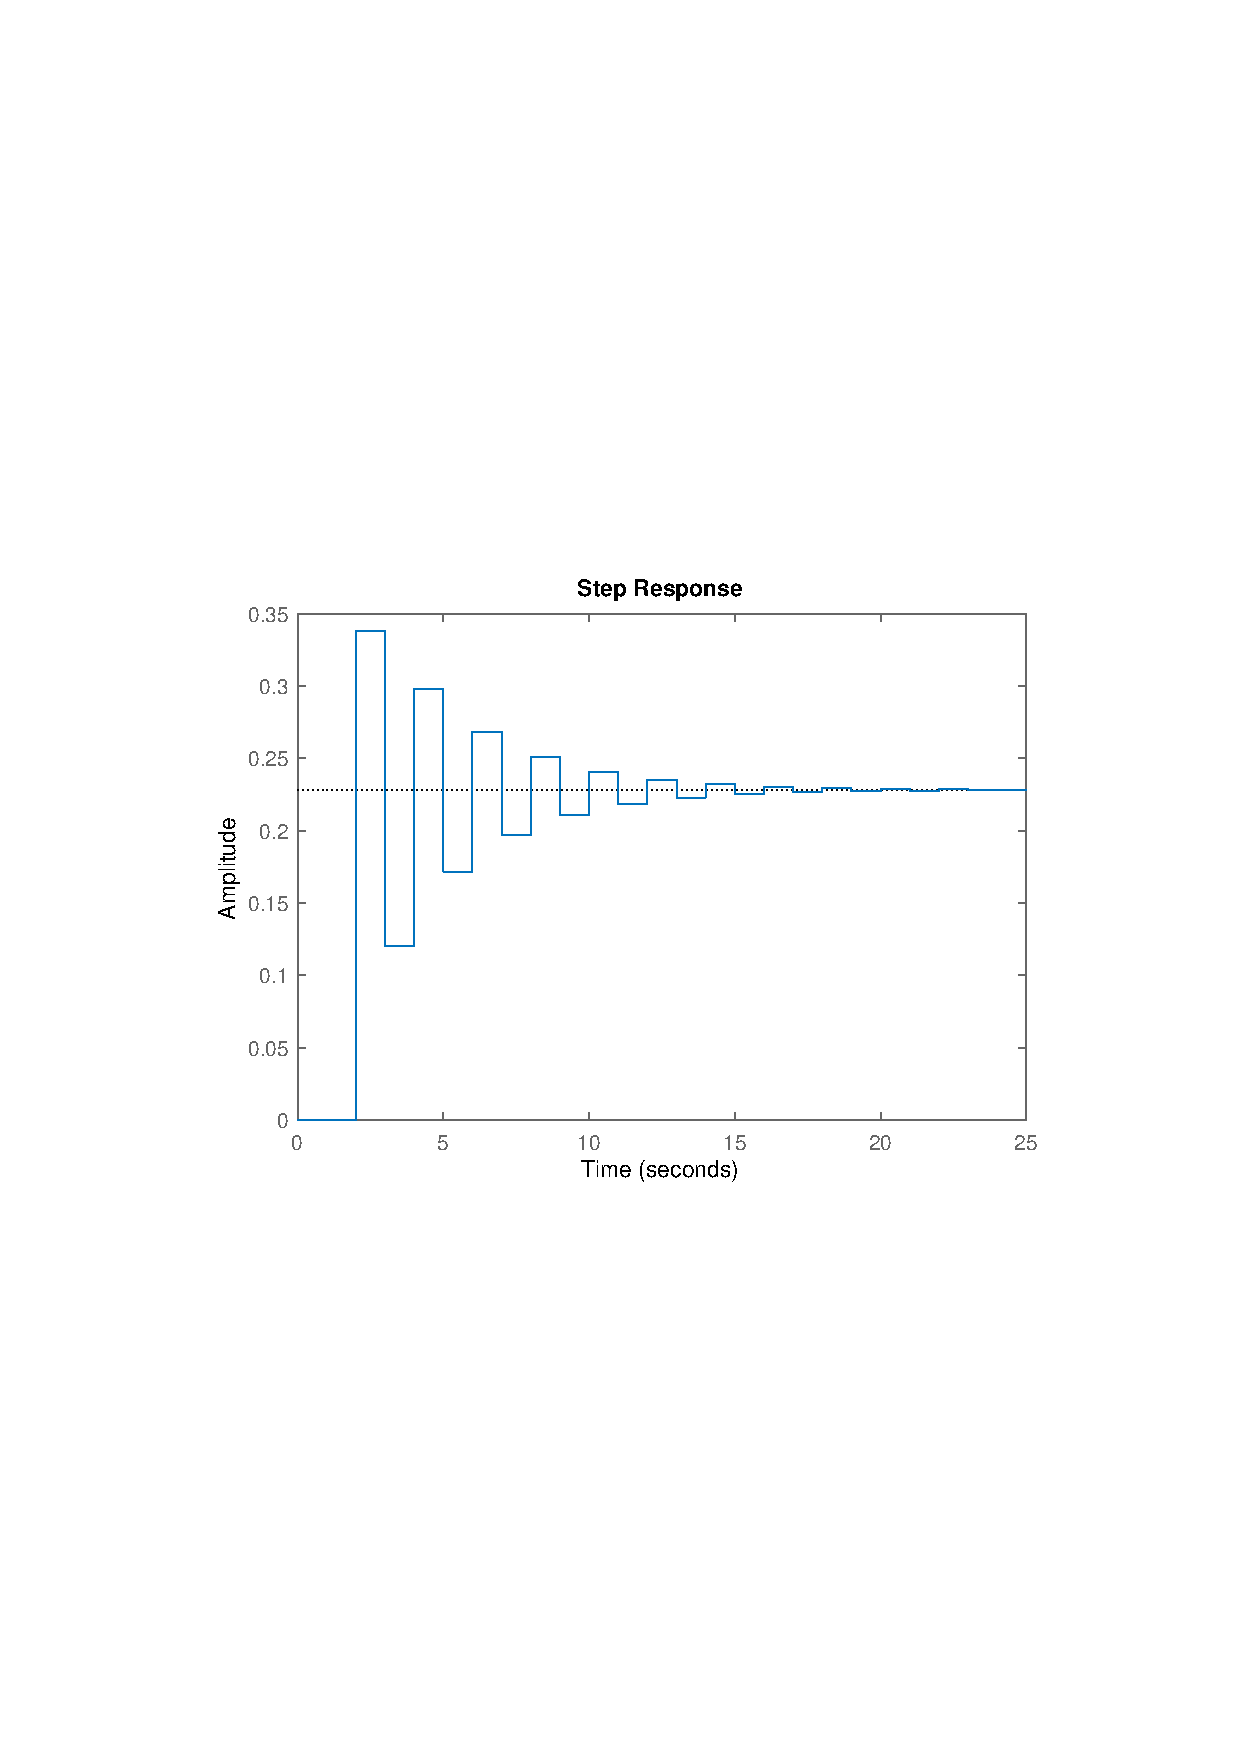
\includegraphics[trim= 10cm 8cm 10cm 8cm, scale=0.4]{figures/1b-step.pdf}
	\caption{Step response using ltiview}
	\label{fig:1b-step}
\end{subfigure}
\caption{MATLABs build in function \emph{ltiview} analyzing the found ARX model for the system in \eqref{eq:system} including noise.}
\label{fig:1b-ltiview}
\end{figure}

\fi


\end{document}
